%
% frames.tex
%
% (c) 2019 Prof Dr Andreas Müller, Hochschule Rapperswil
%
\section{Frames
\label{section:frames}}
\rhead{Frames}
Eine orthonormierte Basis eines Hilbertraumes ist sehr starr.
Es ist nicht möglich, auch nur einen einzigen Vektor ein kleines
Bisschen zu ändern, ohne die Eigenschaften, die zum Satz~\ref{satz:parseval}
geführt haben, zu zerstören.
Im Hinblick auf die numerische Behandlung von Signalen ist das
ein unerwünschter Zustand.
Rundungsfehler werden unvermeidlich dazu führen, dass solche strengen
Strukturen nur näherungsweise im Computer nachgebildet werden 
können.

Die Zerlegung eines Vektors $v$ in einer Orthonormalbasis enthält keine
Redundanz.
Geht einer der Koeffizienten $\hat{v}_k$ verloren, gibt es keine
Chance, den Vektor zu rekonstruieren.
Auch diese Situation ist unerwünscht, denn durch Rundungsfehler geht
mindestens ein Teil der Information in einem Koeffizienten verloren.
Wir suchen daher nach einer Verallgemeinerung des Basis-Begriffs, welche
auf kontrollierte Weise Redundanz in die Koeffizienten $\hat{v}_k$
bringt und damit eine robustere Konstruktion ermöglicht.

%
% Geometrisches Beispiel für ein Frame
%
\subsection{Ein geometrisches Beispiel
\label{subsection:hexagon}}
\begin{figure}
\centering
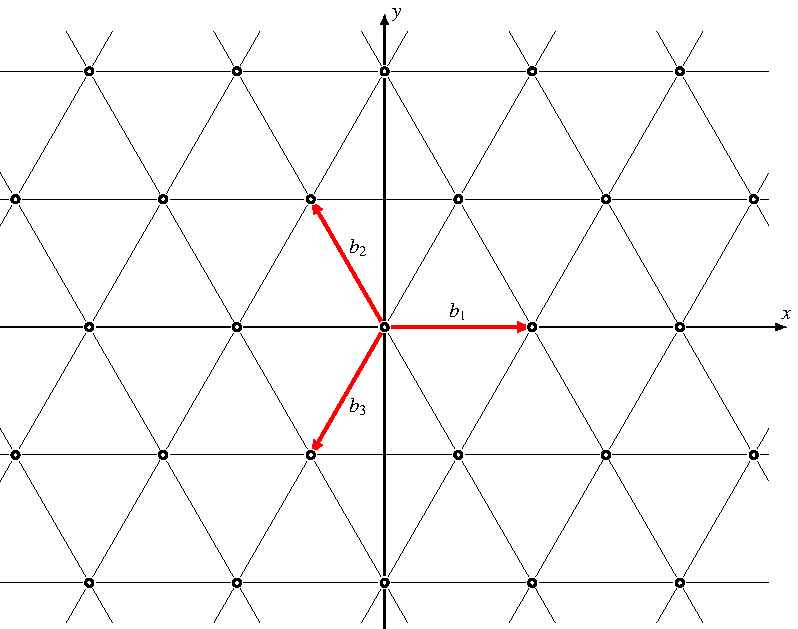
\includegraphics{chapters/1-geometrie/images/hexagon.pdf}
\caption{Sechseck-Gitter in der Ebene zum Frame $\{b_1,b_2,b_3\}$.
\label{geometrie:hexagon:image}}
\end{figure}
Wir suchen ein geeignetes Koordinatensystem, um ein Problem über
Bienenwaben in der Ebene zu lösen.
Dazu gehört das hexagonale Gitter in Abbildung~\ref{geometrie:hexagon:image}.
Selbstverständlich kann dafür das übliche rechtwinklige Koordinatensystem
verwendet werden, aber die Ecken eines Sechsecks shaben darin die nicht
sehr symmetrischen Koordinaten
\begin{center}
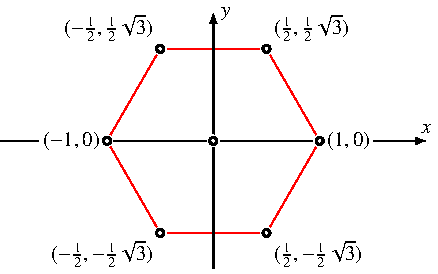
\includegraphics{chapters/1-geometrie/images/hexagon1.pdf}
\end{center}
(Siehe auch Abbildung~\ref{geometrie:hexagon:image}).
Eine bessere Variante ist das Koordinatensystem auf der Basis der beiden
Basisvektoren (in kartesischen Koordinaten)
\[
b_1 = \begin{pmatrix} 1\\0\end{pmatrix}
\qquad
\text{und}
\qquad
b_2 = \begin{pmatrix} -\frac12\\\frac12\sqrt{3}\end{pmatrix}.
\]
In diesem Koordinatensystem haben die Ecken des Sechsecks die Koordinaten
\begin{center}
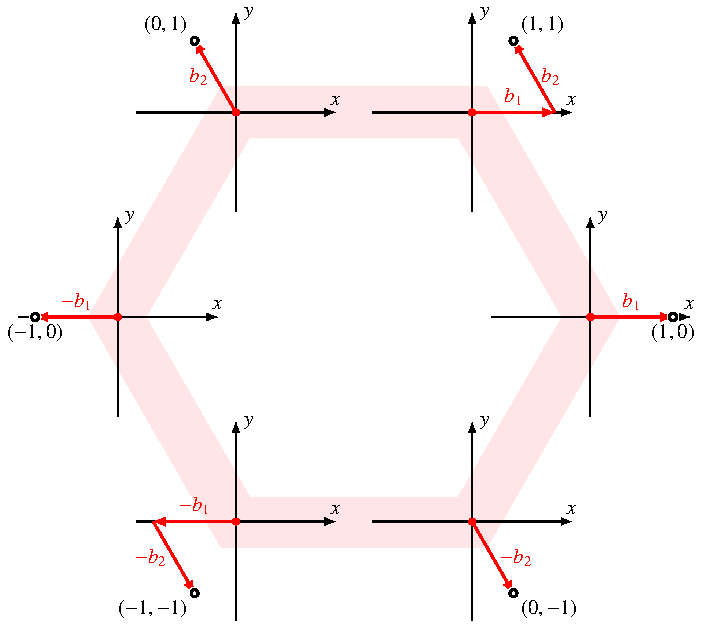
\includegraphics{chapters/1-geometrie/images/hexagon2.pdf}
\end{center}
%\begin{center}
%\begin{tikzpicture}
%\def\a{1.8}
%\foreach \p in {0,60,...,360}{
%	\draw[line width=0.1pt] ({\a*cos(\p)},{\a*sin(\p)})--
%		({\a*cos(\p+60)},{\a*sin(\p+60)});
%}
%\foreach \p in {0,60,...,300}{
%	\fill[color=white] ({\a*cos(\p)-0.65},{\a*sin(\p)-0.25})
%		rectangle ({\a*cos(\p)+0.65},{\a*sin(\p)+0.25});
%}
%
%\node at (0,0) {$0$};
%\node at ({\a},0) {$(1,0)$};
%\node at ({-\a},0) {$(-1,0)$};
%\node at ({0.5*\a},{\a*sqrt(3)/2}) {$(1,1)$};
%\node at ({0.5*\a},{-\a*sqrt(3)/2}) {$(0,-1)$};
%\node at ({-0.5*\a},{\a*sqrt(3)/2}) {$(0,1)$};
%\node at ({-0.5*\a},{-\a*sqrt(3)/2}) {$(-1,-1)$};
%\end{tikzpicture}
%\end{center}
%\begin{align*}
%&      &&(0,1)  &&(1,1)&&     \\
%&(-1,0)&&       &&      &&(1,0)\\
%&      &&(-1,-1)&&(0,-1)&&
%\end{align*}
Was bereits viel besser aussieht.
Trotzdem ist auch dies noch nicht ganz zufriedenstellend. 
Zum Beispiel sind die Ecken links oben und rechts unten direkt durch den
Basisvektor $b_2$ darstellbar, die Ecken rechts oben und links unten
dagegen nur durch eine Linearkombination.
Wir könnten natürlich auch die linke untere Ecke als Basisvektor nehmen,
dann würde eiinfach die linke obere Ecke speziell.
In dieser Situation lässt es sich also mit einer Basis gar nicht erreichen,
dass alle Eckpunkte sich auf einfache Art darstellen lassen.

Verzichten wir jedoch daruf, dass die Vektoren linear unabhängig sein müssen,
können wir als ``Basis'' die drei Vektoren (in kartesischen Koordinaten)
\begin{align}
b_1
&=
\begin{pmatrix}1\\0\end{pmatrix}
&
b_2
&=
\begin{pmatrix}-\frac12\\\frac12\sqrt{3}\end{pmatrix}
&
b_3
&=
\begin{pmatrix}-\frac12\\-\frac12\sqrt{3}\end{pmatrix}
\label{hexagonbasis}
\end{align}
verwenden.
Die drei Vektoren haben alle die Länge $1$, aber sie sind nicht
orthogonal, sondern haben das Skalarprodukt
\[
\langle b_j,b_k\rangle
=
\begin{cases}
-\frac12&\qquad j\ne k\\
1&\qquad j=k.
\end{cases}
\]
Zu jedem Vektor $v\in\mathbb R^2$ können wir wieder eie Koeffizienten
$\hat{v}_k=\langle v,b_k\rangle$ berechnen und damit die Linearkombination
\[
v' = \sum_{k=1}^3 \hat{v}_k\,b_k
\]
bilden,
doch es ist $v\ne v'$.
Wir berechnen die Synthese für die Basisvektoren:
\begin{align*}
b_1'
&=
b_1 - \frac12 b_2 - \frac 12 b_3
=
\frac32b_1
\\
b_2'
&=
-\frac12 b_1 + b_2 -\frac12 b_3
=
\frac32b_2
\\
b_3'
&=
-\frac12b_1-\frac12 b_2 + b_3
=
\frac32b_3
\end{align*}
Die Synthese liefert also nicht den ursprünglichen Vektor, sondern
\begin{equation}
\sum_{k=1}^3 \hat{v}_k b_k = \frac32\,v
\label{geometrie:32beispiel}
\end{equation}
zurück, das $\frac32$-fache davon.
Dies ist bereits ein Ausdruck der Tatsache, dass die Information in den
Koeffizienten $\hat{v}_k$ redundant ist.
Andererseits zeigt dies auch, dass alle Richtungen gleichermassen
verzerrt werden.

Diese Vektoren sind natürlich nicht mehr linear unabhängig, Vektoren
der Ebene können also auf verschieden Art linear aus den $b_k$ kombiniert
werden.
Da $b_1+b_2+b_3=0$ ist, kann man zu den Koeffizienten $\hat{v}_k$
eine beliebige Zahl $\alpha$ hinzuaddieren, und erhält
\[
\sum_{k=1}^3 (\hat{v}_k+\alpha)\, b_k
=
\sum_{k=1}^3 \hat{v}_k\,b_k
+\alpha
\sum_{k=1}^3 b_k
=
\sum_{k=1}^3 \hat{v}_k\,b_k
=
\frac32 v.
\]
Die modifizierten Koeffizienten ergeben also das gleichen synthetisierten
Vektor $\frac32 v$.

Für die Norm des synthetisierten Vektors gilt natürlich
\[
\|v'\|^2
=
\frac94\|v\|^2
=
\sum_{k=1}^3 \hat{v}_k^2 
-
\frac12\sum_{k\ne l} \hat{v}_k\hat{v}_l.
\]
%Die modifizierten Koeffizienten ergeben natürlich dieselbe Norm, also
%\begin{align*}
%\|v'\|^2
%&=
%\sum_{k=1}^3 (\hat{v}_k+\alpha)^2 
%-
%\frac12\sum_{k\ne l} (\hat{v}_k+\alpha)(\hat{v}_l+\alpha).
%\\
%&=
%\sum_{k=1}^3 \hat{v}_k^2
%+2\alpha \sum_{k=1}^3 \hat{v}_k
%+3\alpha^2
%-
%\frac12\sum_{k\ne l} \hat{v}_k\hat{v}_l
%-
%\sum_{k\ne l} \hat{v}_k \alpha
%-
%3\alpha^2
%\end{align*}


Was zeichnet die Koeffizienten $\hat{v}_k$ gegenüber den modifizierten
Koeffiziente $\hat{v}_k$ aus?
In Abbildung~\ref{3dbasisbild} sind die Koeffizienten $\hat{v}_k$ als
dreidimensionaler Vektor $v'$ dargestellt.
Punkte in der Ebene werden durch die Analyse mit Hilfe der Vektoren $b_k$
auf Vektoren in der hellblau hervorgehobenen Ebene abgebildet.
Die alternativen Linearkombinationen entstehen, indem man zu $v$
ein Vielfaches des grünen Normalenvektors $n$ hinzuaddiert.
Die gelb gezeichneten Punkte $w$ bilden eine Gerade senkrecht
auf der hellblauen Ebene.
Alle Punkte auf dieser Geraden führen auf die gleiche
Linearkombination $\frac32v$.
Die mit Hilfe der Skalarprodukte gefundene Linearkombination
$\hat{v}_k=\langle v,b_k\rangle$ hat daher die Eigenschaft, 
$v'$ unter all den Punkte auf der Geraden die kürzeste Länge hat.
Oder: die Koeffizienten $\hat{v}_k$ zeichnen sich unter allen
Koeffizienten $v_k$ mit der gleichen Linearkombination dadurch aus, 
dass
\begin{equation}
\|v'\|^2
=
\sum_{k=1}^n |\hat{v}_k|^2
\le
\sum_{k=1}^n |v_k|^2
\qquad
\text{für Koeffizienten $v_k$ mit}
\quad
\sum_{k=1}^3 \hat{v}_kb_k
=
\sum_{k=1}^3 v_kb_k
\label{hexagonbasiseigenschaft}
\end{equation}
ist.
Die durch $\hat{v}_k$ gefundenen Koeffizienten zeichnen sich durch
die minimale ``Koeffizientenenergie'' aus.

Im Falle einer Orthonormalbasis konnte man dank der Plancherel-Formel
die Norm eines Vektors mit Hilfe der Quadratsumme der Koeffizienten
berechnen.
Die Eigenschaft \eqref{hexagonbasiseigenschaft} kann also als erweiterte
Form der Plancherel-Formel angesehen werden.

\begin{figure}
\centering
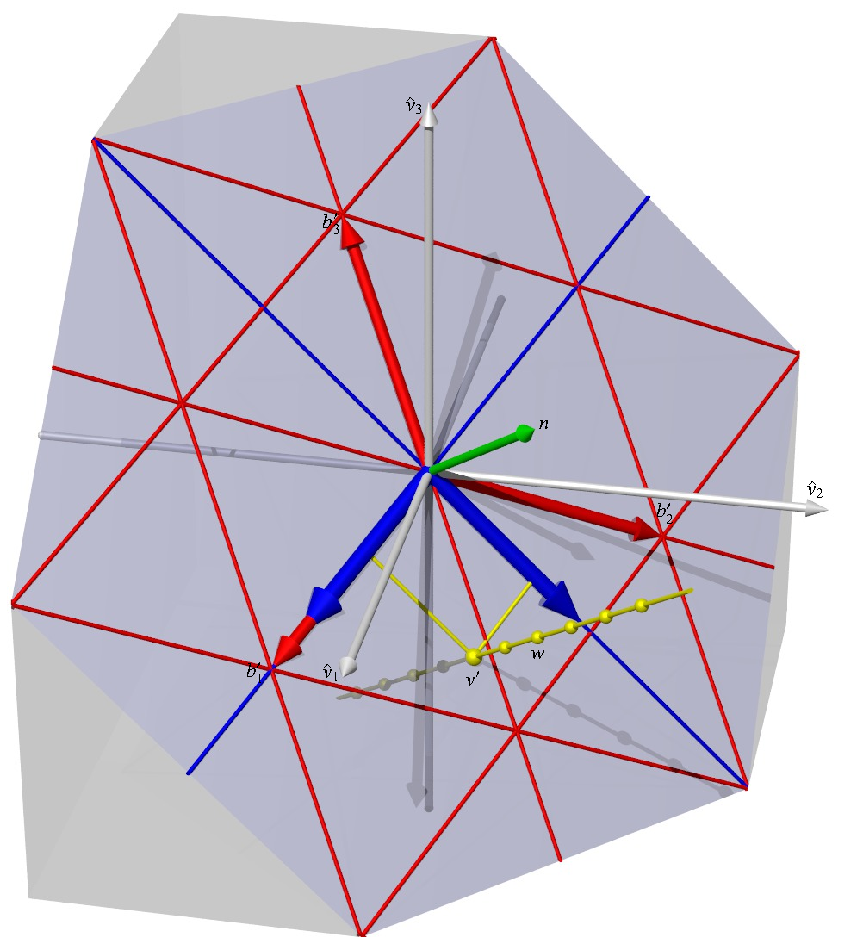
\includegraphics{chapters/1-geometrie/images/tri.pdf}
\caption{Darstellung der Koeffizienten $\hat{v}_k$ bezüglich Vektoren $b_i$
aus \eqref{hexagonbasis}.
Die drei Vektoren $b_i$ haben als $\hat{v}_k$-Koeffizienten-Vektoren
die Vektoren $b_i'$.
Die $x$- und $y$-Achsrichtung werden auf die beiden blauen Vektoren
abgebildet.
Ein Vektor $v$ wird auf den Vektor $v'$ mit den Komponenten
$\hat{v}_k$ abgebildet.
Die Darstellung eines Vektors als Linearkombination der $b_i$ ist
jedoch nicht eindeutig.
Ändert man die Koeffizienten um den gleichen Wert, was gleichbedeutend damit
ist, dass man dem Vektor $v'$ ein Vielfaches von $n$ hinzufügt, entsteht
bei der Synthese $\sum \hat{v}_k b_k$ der gleiche Punkt.
Alle gelben Punkte $w$ sind daher Koeffizienten, die den gleichen Punkt $v$
ergeben, wenn man damit die Vektoren $b_i$ linear kombiniert.
\label{3dbasisbild}}
\end{figure}

%
% Definition eines Frames
%
\subsection{Definition eines Frames}
Nach dem motivierenden Beispiel im vorangegangenen Abschnitt sind wir nun
bereit, eine allgemeine Definition aufzubauen.
Wir wollen also weiterhin die Vektoren eines Vektorraums $V$ mit Hilfe
einer Menge von Vektoren $\{e_k\,|\,1\le k\le n\}$ linear kombinieren,
verlangen aber nicht mehr, dass die Vektoren $e_k$ linear unabhängig sind.
Dies bedeutet natürlich, dass die Darstellung eines Vektors $v\in V$
nicht mehr eindeutig sein wird.

Nicht jede Menge von Vektoren $\{e_k\,|\,1\le k\le n\}$ ist geeignet.
Es muss ja immer noch jeder Vektor dargestellt werden können, das
Erzeugnis $U := \langle e_k\,|\,1\le k\le n\rangle$
der Vektoren muss also der ganze Vektorraum sein:
\[
U
=
V.
\]
Wäre das Erzeugnis nur ein echter Unterraum $U\subset V$, dann gäbe es
einen Vektor $b\in V$, der senkrecht steht auf allen $b\perp U$.
Wir fordern daher, dass es keinen Vektor gibt, der auf allen Vektoren $e_k$
senkrecht steht.

Damit die Berechnung effizient bleibt, möchten wir weiterhin nur mit den
Koeffizienten $\hat{v}_k = \langle v,e_k\rangle$ arbeiten können.
Für eine Orthonormalbasis hat die Plancherel-Formel gezeigt, dass
\[
\sum_{k=1}^n |\hat{v}_k|^2 = \| v \|.
\]
In der aktuellen Situation können wir nicht mehr erwarten, dass dies 
weiterhin funktioniert.
Wir müssen aber mindestens verlangen, dass die Transformation
\[
\mathcal{T}
\colon
V\to \mathbb R^n
:
v\mapsto \hat{v}_k
\]
stetig ist, dass sich also kleine Änderungen von $v$ ebenfalls
kleinen Änderungen des Vektors der $\hat{v}_k$ auswirken.
Es muss also eine Konstante $B$ geben, so dass
\[
\sum_{k=1}^n |\hat{v}_k|^2
=
\sum_{k=1}^n |\langle v,e_k\rangle|^2
\ge
A \| v \|^2.
\]

Wir müssen aber auch sicherstellen, dass die Rekonstruktion des Vektors $v$
auf stetige Art von den Koeffizienten $\hat{v}_k$ abhängt. 
Eine kleine Änderung der Koeffizienten darf sich nur in beschränkten Änderungen
im rekonstruierten Vektor $v$ auswirken.
Es muss also eine Konstante $B$ geben, so dass
\[
\sum_{k=1}^n |\hat{v}_k|^2
=
\sum_{k=1}^n |\langle v,e_k\rangle|^2
\le
B \| v \|^2
\]
gilt.

Damit haben wir alle Elemente zusammen für die folgende Definition,
die auch für unendlichdimensionale Hilberträume funktioniert.

\begin{definition}
\label{definition:frame}
Eine Teilmenge $\{ e_k\,|\, k\in K\}\subset V$ heisst ein {\em Frame},
wenn es zwei positive Konstanten $A>0$ und $B>0$ gibt, so dass
\[
A\|v\|^2 \le \sum_{k\in K} |\langle v, e_k\rangle|^2 \le B \| v\|^2
\]
gilt für jeden Vektor $v\in V$.
Die Konstanten $A$ und $B$ heissen die {\em Framekonstanten} des Frames.
Das Frame heisst {\em straff}, wenn $A=B$ ist.
\end{definition}

\begin{beispiel}
Das Beispiel von Abschnitt~\ref{subsection:hexagon} ist ein Frame.
Die Formel \eqref{geometrie:32beispiel} zeigt, dass die Framekonstanten
des Frames $A=B=\frac32$ ist.
Das Frame ist also sogar straff.
\end{beispiel}

In der Definition wird nicht erwähnt, dass die Vektoren des Frames den
ganzen Raum aufspannen müssen.
Diese Eigenschaft folgt jedoch direkt aus der Definition eines Frames,
wie der folgende Satz zeigt.

\begin{satz}
Ist $\mathcal{B}=\{ e_k\,|\, k\in K\}$ ein Frame des Hilbertraumes $V$
mit Framekonstanten $A$ und $B$, dann gibt es keinen Vektor $v\in V$,
der auf allen Vektoren $e_k$ senkrecht steht.
\end{satz}

\begin{proof}[Beweis]
Nehmen wir an, es gäbe einen Vektor $v\in V$ mit $\langle v,e_k\rangle=0$
für alle $k\in K$.
Dann folgt aus den Frame-Ungleichungen
\[
\| v \|^2 \le \frac1{A} \sum_{k\in K} |\langle v,e_k\rangle|^2 = 0
\qquad\Rightarrow\qquad
v=0.
\]
Der Nullvektor ist also der einzige Vektor, der auf allen Framevektoren
senkrecht steht.
\end{proof}

Eine orthonormierte Basis war die bevorzugte Wahl für eine Basis, weil
sich damit die Transformation $\mathcal{T}$ besonders leicht invertieren
lässt.
Der Satz~\ref{satz:parseval} hat gezeigt, dass die Transformation %$\mathcal{T}$
eine Isometrie ist, insbesondere gilt
\[
\|v\|^2
=
\sum_{k\in K} |\hat{v}_k|^2
=
\sum_{k\in K} |\langle v,e_k\rangle|^2.
\]
Dies bedeutet, dass eine orthonormierte Basis ein straffes Frame mit
Framekonstanten $A=B=1$ ist.
Umgekehrt drängt sich die Frage auf, ob straffe Frames oder spezielle
Werte der Frame-Konstanten eine besondere Bedeutung für die Invertierbarkeit
haben.

\begin{figure}
\centering
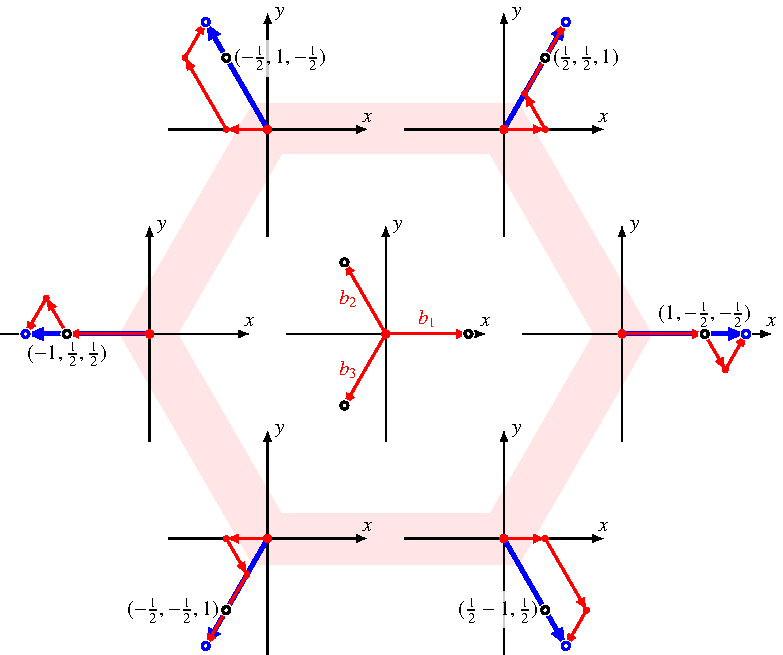
\includegraphics{chapters/1-geometrie/images/hexagon3.pdf}
\caption{Rekonstruktion bei einem straffen Frame.
Das Frame bestehend aus den Vektoren $\{b_1,b_2,b_3\}$ ist straff
mit der Framekonstanten $A=\frac32$.
Die mit den Skalarprodukten gewichtete Linearkombination der
Framevektoren liefert nicht den ursprünglichen Vektor zurück, sondern
einen Vektor, der mit der Framekonstanten multipliziert wird.
Gezeigt wird dies für die sechs Ecken des Hexagons.
Die Skalarprodukte mit den Framevektoren, die Framekoordinaten, sind
als Zahlentripel bei jedem Punkt angegeben.
Die roten Vektorpfade stellen die Linearkombination dar, die blauen
Vektoren die Summe.
\label{geometrie:hexagon:rekonstruktion}}
\end{figure}

%
% Frames in R^n
%
\subsection{Frames in $\mathbb R^n$
\label{subsetion:skript:frames:framesinrn}}
Wir betrachten jetzt den Spezialfall $H=\mathbb{R}^n$ mit dem
Standardskalarprodukt.
Jeder endlichdimensionale Hilbertraum lässt sich durch Wahl einer
Orthonormalbasis in dieser Form beschreiben.
Das Beispiel von Abschnitt~\ref{subsection:hexagon} ist ein Beispiel für
den Fall $\mathbb R^2$.

Ein Frame in $\mathbb R^n$ ist nach Definition~\ref{definition:frame}
eine Menge 
\[
\mathcal{B}
=
\{b_1,\dots,b_m\}
\subset
\mathbb R^n
\]
von Vektoren in $\mathbb R^n$ mit zwei positiven Konstanten $A$ und $B$
derart, dass
\[
A\|v\|^2
\le
\sum_{k=1}^m |\langle v,b_k\rangle|^2
\le
B\|v\|^2
\]
gilt für jeden Vektor $v\in\mathbb R^n$.
Da alle beteiligten Vektorräume endlichdimensional sind, können
die Abbildungen als Matrizen beschrieben werden.
Ziel dieses Abschnitts ist, neben einer Matrizenbeschreibung
der Frame-Abbildung $\mathcal{T}$ auch eine Formel für die
Umkehrabbildung zu finden.

In einem endlichdimensionalen Raum ist die Frame-Bedingung $A>0$ 
gleichbedeutend damit, dass die Frame-Vektoren den ganzen Raum erzeugen.

\subsubsection{Der Frame-Operator}
Der Frame-Operator berechnet die Analysekoeffizienten
$\hat{v}_k=\langle v,b_k\rangle$ eines Signals
$v\in \mathbb R^n$ bezüglich des Frames $\mathcal{B}$:
\[
\mathcal{T}\colon \mathbb R^n \to \mathbb R^m
:
v \mapsto
\begin{pmatrix}
\hat{v}_1\\\hat{v}_2\\\vdots\\\hat{v}_m
\end{pmatrix}
=
(\hat{v}_k=\langle v,b_k\rangle)_{1\le k\le m}.
\]
Zur Berechnung der Skalarprodukte kann man das Matrizenproukt
\[
\langle v,b_k\rangle
=
b_k^t v
\]
verwenden.
Die Zeilenvektoren $b_k^t$ kann man zeilenweise in einer grossen Matrix $T$
\[
T 
=
\begin{pmatrix}
\dots&b_1^t &\dots\\
\dots&b_2^t &\dots\\
     &\vdots&     \\
\dots&b_m^t &\dots
\end{pmatrix}
\]
zusammenführen.
Das Matrixprodukt $Tv$ liefert dann genau das Resultat des Frame-Operators
\[
\mathcal{T} v
=
\begin{pmatrix}
\langle v, b_1\rangle\\
\langle v, b_2\rangle\\
\vdots\\
\langle v, b_m\rangle\\
\end{pmatrix}
=
\begin{pmatrix}
b_1^tv\\
b_2^tv\\
\vdots\\
b_m^tv\\
\end{pmatrix}
=
\begin{pmatrix}
\dots&b_1^t &\dots\\
\dots&b_2^t &\dots\\
     &\vdots&     \\
\dots&b_m^t &\dots
\end{pmatrix}
v
=
Tv.
\]
Die Matrix $T$ ist die Matrix des Frame-Operator $\mathcal T$ bezüglich der
Standardbasis von $\mathbb R^n$.

\begin{beispiel}
Im Beispiel von Abschnitt~\ref{subsection:hexagon} besteht das Frame
aus den Vektoren
\[
\mathcal{B}
=
\biggl\{
\begin{pmatrix}1\\[2pt] 0\end{pmatrix},
\begin{pmatrix}-\frac12\\[2pt] \frac{\sqrt{3}}2\end{pmatrix},
\begin{pmatrix}-\frac12\\[2pt] -\frac{\sqrt{3}}2\end{pmatrix}
\biggr\}.
\]
Der zugehörige Frameoperator $\mathcal{T}$ hat daher die Matrix
\begin{equation}
T
=
\begin{pmatrix}
1&0\\[2pt]
-\frac12&\frac{\sqrt{3}}2\\[2pt]
-\frac12&-\frac{\sqrt{3}}2
\end{pmatrix}.
\label{beispielTmatrix}
\end{equation}
\end{beispiel}

\subsubsection{Die Gram-Matrix}
Das Frame $\mathcal{B}$ mit den Frame-Konstanten $A$ und $B$ erfüllt
\[
A\|v\|^2 \le \sum_{k=1}^m |\langle v,b_k\rangle|^2 \le B\|v\|^2
\qquad\forall v\in \mathbb R^n.
\]
Die Quadratsumme in der Mitte ist genau die Norm des Vektors
$\mathcal{V}$ in $\mathbb R^m$.
Unterscheiden wir für den Moment die verschiedenen Skalarprodukte
und Normen dadurch, dass wir die Vektorräume als Indizes hinzufügen,
können wir die Frame-Ungleichung schreiben als
\[
A \| v\|_{\mathbb R^n}^2
\le
\| Tv\|_{\mathbb R^m}^2
\le
B \| v\|_{\mathbb R^n}^2.
\]
Die Norm von $Tv$ in $\mathbb R^m$ ist
\[
\| Tv\|_{\mathbb R^m}^2
=
\langle Tv,Tv\rangle_{\mathbb R^m}
=
(Tv)^tTv
=
v^t(T^tT)v
=
\langle T^tTv,v\rangle_{\mathbb R^n}.
\]
Man beachte, dass $T^tT$ eine symmetrische $n\times n$-Matrix ist,
die codiert, wie stark die einzelnen Vektoren $v\in\mathbb R^n$ durch
den Frame-Operator $\mathcal{T}$ verzerrt werden.
Dies rechtfertigt eine eigene Definition.

\begin{definition}
Ist $T$ die Matrix des Frame-Operators $\mathcal{T}$ eines Frames
$\mathcal{B}$, dann heisst $G=T^tT$ der Gram-Operator des Frames
$\mathcal{B}$.
\end{definition}

Die Frame-Bedingung lässt sich mit dem Gram-Operator $T^tT$ als
\begin{equation}
A \|v\|^2
\le
\langle T^t T v,v\rangle
\le
B \|v\|^2
\label{framebedingung:ttt}
\end{equation}
schreiben.
Man kann daraus schliessen, dass der Gram-Operator $T^tT$ regulär ist.

Die symmetrische Matrix $T^tT$ kann durch Wahl einer geeigneten Basis
in $\mathbb R^n$ diagonalisiert werden.
Die Eigenvektoren können sogar orthonormiert gewählt werden.
Seien daher $u_1,\dots,u_n$ Eigenvektoren von $T^tT$ mit Eigenwerten
$\lambda_1\le\dots\le\lambda_n$.
Die Framebedingung~\eqref{framebedingung:ttt}
für den Vektore $v=u_k$ sagt dann
\[
A \| u_k\|^2
=
A
\le
\langle T^tTu_k,u_k\rangle
=
\lambda_k\langle u_k,u_k\rangle
=
\lambda_k
=
B \| u_k\|^2
=
B.
\]
Die Eigenwerte von $T^tT$ sind also alle zwischen $A$ und $B$.
Man kann sogar noch mehr sagen:

\begin{satz}
Sei $\mathcal{B}\subset\mathbb R^n$ eine Menge von Vektoren derart,
dass die zugehörige Matrix $T^tT$ regulär ist.
Seien weiter $\lambda_1\le\dots\le \lambda_n$ die Eigenwerte
(mit Vielfachheiten) von $T^tT$.
Dann ist $\mathcal{B}$ ein Frame mit Framekonstanten
$A=\lambda_1$ und $B=\lambda_n$.
\end{satz}

\begin{beispiel}
Im Beispiel von Abschnitt~\ref{subsection:hexagon} ist die Matrix $T$
gegeben in \eqref{beispielTmatrix}.
Der zugehörige Gram-Operator ist
\[
T^tT
=
\begin{pmatrix}
1& -\frac12        &-\frac12          \\[2pt]
0& \frac{\sqrt{3}}2& -\frac{\sqrt{3}}2
\end{pmatrix}
\begin{pmatrix}
1&0\\
-\frac12&\frac{\sqrt{3}}2\\[2pt]
-\frac12&-\frac{\sqrt{3}}2
\end{pmatrix}
=
\begin{pmatrix}
1+\frac14+\frac14 & 0-\frac{\sqrt{3}}4+\frac{\sqrt{3}}4\\[2pt]
0-\frac{\sqrt{3}}4+\frac{\sqrt{3}}4&0+\frac{3}{4}+\frac{3}{4}
\end{pmatrix}
=
\begin{pmatrix}
\frac32&0\\
0&\frac32
\end{pmatrix}
=
\frac{3}{2}E
\]
Da die Matrix $T^tT$ bereits diagonal ist, können die Eigenwerte
$\lambda_1=\lambda_2=\frac32$ direkt abgelesen werden.
\end{beispiel}

Das Frame des Beispiels ist straff und der Gram-Operator ist ein
Vielfaches der Einheitsmatrix.
Dies ist kein Zufall, wie das folgende Korollar zeigt.

\begin{korollar}
Das Frame $\mathcal{B}$ ist genau dann straff, wenn der zugehörige
Gram-Operator $T^tT$ ein Vielfaches der Einheitsmatrix ist.
\end{korollar}

\begin{figure}
\centering
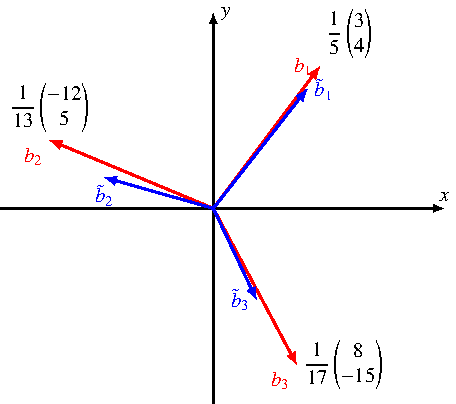
\includegraphics{chapters/1-geometrie/images/beispiel2.pdf}
\caption{Beispiel eines nicht straffen Frames mit rationalen Framevektoren
$b_k$ (rot).
Die Vektoren $\tilde{b}_k$ des dualen Frames
(siehe Definition~\ref{definition:dualesframe}) sind blau eingezeichnet.
\label{frame:beispiel2}}
\end{figure}

\begin{beispiel}
Die Vektoren
\[
\mathcal{B} 
=
\biggl\{
\frac15
\begin{pmatrix} 3\\4\end{pmatrix},
\frac1{13}
\begin{pmatrix} -12\\5\end{pmatrix},
\frac1{17}
\begin{pmatrix} 8\\-15\end{pmatrix}
\biggr\}
\subset \mathbb R^2
\]
erzeugen den ganzen Raum $\mathbb R^2$, sie bilden daher ein
Frame (Abbildung~\ref{frame:beispiel2}).
Wir berechnen den Frame-Operator, den Gram-Operator und seine Eigenwerte
um die Frame-Konstanten zu ermiteln.

Der Frame-Operator ist die Matrix
\[
T
=
\begin{pmatrix}
 \frac{ 3}{ 5}& \frac{ 4}{ 5}\\[2pt]
-\frac{12}{13}& \frac{ 5}{13}\\[2pt]
 \frac{ 8}{17}&-\frac{15}{17}
\end{pmatrix}.
\]
Der Gram-Operator wird daher
\[
G=T^tT
=
\begin{pmatrix}
 \frac{ 3}{ 5}&-\frac{12}{13}&  \frac{ 8}{17}\\[2pt]
 \frac{ 4}{ 5}& \frac{ 5}{13}& -\frac{15}{17}
\end{pmatrix}
\begin{pmatrix}
 \frac{ 3}{ 5}& \frac{ 4}{ 5}\\[2pt]
-\frac{12}{13}& \frac{ 5}{13}\\[2pt]
 \frac{ 8}{17}&-\frac{15}{17}
\end{pmatrix}
=
\frac{1}{1221025}
\begin{pmatrix}
1750369&  286808 \\
 286808& 1676106
\end{pmatrix}
\]
Die Eigenwerte dieser $2\times 2$-Matrix können als Nullstellen des
charakteristischen Polynoms mit der Lösungsformel für quadratische
Gleichungen berechnet werden.
Man findet zum Beispiel mit Hilfe eines Computer-Algebra-Systems
\[
\lambda_{\pm}
=
\frac{52715\pm 41\sqrt{47105}}{37570}
\quad\Rightarrow\quad
\left\{
\begin{aligned}
A&=
1.166262672548251
\\
B&=
1.639965701154171.
\end{aligned}
\right.
\]
Da die beiden Konstanten nicht übereinstimmen, ist dieses Frame
nicht straff.
\end{beispiel}

\begin{proof}[Beweis]
Ein straffes Frame hat $A=B$, was gleichbedeutend damit ist, dass
die Eigenwerte des Frame-Operators $T^tT$ mit 
$A=B=\lambda_1=\dots=\lambda_n$ übereinstimmen.
Dies wiederum ist gleichbedeutend damit, dass alle Vektoren Eigenvektoren
zum gleichen Eigenwert sind und $T^tT=AE=BE$.
\end{proof}

\subsubsection{Die inverse Abbildung des Frame-Operators}
Für ein straffes Frame gilt $T^tT  = AE$.
Bis auf den Faktor $A$ ist daher $T^t$ bereits eine Linksinverse von $T$.
Genauer, mit
\[
S=\frac1{A} T^t
\qquad\text{folgt}\qquad
ST
=
\frac1{A} T^tT
=
\frac1{A} AE
=
E.
\]
Eine Linksinverse von $\mathcal{T}$ ist also für ein straffes Frame
leicht zu finden.

Für ein beliebiges Frame lässt sich ebenfalls eine Linksinverse angeben.
Mit $G=T^tT$ ist
\[
v
=
\underbrace{G^{-1}T^t}_{\displaystyle=S}Tv
=
STv,
\]
die Matrix $S=G^{-1}T^t$ ist also die gesuchte Linksinverse von $T$.

\subsubsection{Das duale Frame}
Um den Frame-Operator umzukehren, muss man $G^{-1}T^t$ berechnen
können.
Auf einen Vektor $\hat{v} = (\hat{v}_k)_{1\le k\le m} = Tv$ angewendet
bedeutet dies, dass man $G^{-1}$ auf
\[
T^t \hat{v} = \sum_{k=1}^m \hat{v}_k  b_k,
\]
anwenden muss, dabei wurde verwendet, dass $T^t$ als Spalten die
Vektoren $b_k$ enthält.
Anwendung von $G^{-1}$ liefert
\[
v
=
G^{-1} T^t \hat{v}
=
\sum_{k=1}^m \hat{v}_k G^{-1}b_k.
\]
Den Vektor $v$ erhält man also als Linearkombination der Vektoren
\[
\tilde{\mathcal{B}}
=
\{ G^{-1}b_1,\dots,G^{-1}b_n\}
=
\{ \tilde{b}_k = G^{-1}b_k\,|\, 1\le k\le m\}.
\]

\begin{definition}
\label{definition:dualesframe}
Ist $\mathcal{B}=\{b_1,\dots,b_m\}$, dann heisst
$\tilde{\mathcal{B}} = \{\tilde{b}_1,\dots,\tilde{b}_m\}$ 
mit
$\tilde{b}_k=G^{-1} b_k$
das zu $\mathcal{B}$ duale Frame.
\end{definition}

\begin{beispiel}
Das duale Frame zum Beispiel zu Abbildung~\ref{frame:beispiel2} kann
ebenfalls mit Hilfe eines Computer-Algebra-Systems berechnet werden aus
der bereits früher berechneten Matrix bestimmt werden.
Aus 
\[
G^{-1}T^t
=
\begin{pmatrix}
\frac{4259}{8053}
	&-\frac{718432}{1167685}
		&\frac{284716}{1167685}\\[2pt]
\frac{5422}{8053}
	&\frac{408473}{2335370}
		&-\frac{1203549}{2335370}
\end{pmatrix}
=
\begin{pmatrix}
0.52887&-0.61526&\phantom{-} 0.24383\\
0.67329&\phantom{-} 0.17490&-0.51536
\end{pmatrix}
\]
findet man das duale Frame
\[
\tilde{\mathcal{B}}
=
\left\{
\begin{pmatrix}
\frac{4259}{8053}\\[2pt]
\frac{5422}{8053}
\end{pmatrix},
\begin{pmatrix}
-\frac{718432}{1167685}\\[2pt]
\frac{408473}{2335370}
\end{pmatrix},
\begin{pmatrix}
\frac{284716}{1167685}\\[2pt]
-\frac{1203549}{2335370}
\end{pmatrix}
\right\}
=
\left\{
\begin{pmatrix} 0.52887\\ 0.67329 \end{pmatrix},
\begin{pmatrix}-0.61526\\ \phantom{-}0.17490 \end{pmatrix},
\begin{pmatrix}\phantom{-}0.24383\\ -0.51536 \end{pmatrix}
\right\}.
\]
Die Vektoren des dualen Frames sind in Abbildung~\ref{frame:beispiel2}
blau eingezeichnet.
\end{beispiel}

\begin{korollar}
Ist $\mathcal{B}=\{b_1,\dots,b_m\}$ ein straffes Frame mit Framekonstanten
$A=B$, dann ist
\[
\tilde{\mathcal{B}}
=
\biggl\{\tilde{b}_k = \frac1Ab_k\,\bigg|\,1\le k\le m\biggr\}
\]
das dazu duale Frame.
\end{korollar}

\begin{proof}[Beweis]
Für ein straffes Frame ist $T^tT=AE$, also ist $G^{-1}=\frac1A E$.
Die Vektoren des dualen Frames sind daher
$\tilde{b}_k = \frac1AEb_k=\frac1Ab_k$.
\end{proof}

Die Linksinverse $S$ von $\mathcal{T}$ kann mit Hilfe des dualen Frames
sehr leicht formuliert werden.

\begin{satz}
Ist $\mathcal{B}$ ein Frame und $\tilde{\mathcal{B}}$ das dazu duale
Frame und ist $\hat{v} = Tv$, dann ist die Linksinverse $S$ von $T$
gegeben durch
\[
v
=
S\hat{v}
=
\sum_{k=1}^m \hat{v}_k \tilde{b}_k.
\]
Linearkombination der Vektoren des dualen Frames mit den Analysekoeffizienten
$\hat{v}_k$ liefert also das ursprüngliche Signal zurück.
\end{satz}

\begin{beispiel}
\label{beispiel3}
In diesem Beispiel betrachten wir das Frame bestehend aus den
Signalen, die auf einem von maximal zehn Samles konstant sind
und sonst verschwinden.
Das Signal $b_k$ verschwindet für Samples $i>k$ und $i<k-10$
und ist so normiert, dass $\|b_k\|=1$.
Die zugehörigen dualen Signale können direkt berechnet werden,
zwei Beispiele sind in den Abbildungen \ref{b3-01} und \ref{b3-05}
dargestellt.
\def\beispieldrei#1#2{
\begin{figure}
\centering
\includegraphics{chapters/1-geometrie/images/b3-#1.pdf}
\caption{Signal $b_{#2}$ aus dem Beispiel von Seite~\pageref{beispiel3}
und zugehöriges duales Signal $\tilde{b}_{#2}$.
\label{b3-#1}}
\end{figure}
}
\beispieldrei{01}{1}
%\beispieldrei{02}{3}
%\beispieldrei{03}{6}
%\beispieldrei{04}{10}
\beispieldrei{05}{20}
%\beispieldrei{06}{30}
%\beispieldrei{07}{40}
%\beispieldrei{08}{50}
%\beispieldrei{09}{60}
%\beispieldrei{10}{70}
\end{beispiel}

In der Definition~\ref{definition:dualesframe} wird das duale Frame
definiert ohne zu rechtfertigen, dass die Vektoren $\tilde{b}_k$ 
tatsächlich ein Frame bilden.
Wegen $b_k=G\tilde{b}_k$ ist aber klar, dass die Vektoren $\tilde{b}_k$
den ganzen Vektorraum $\mathbb R^n$ erzeugen.
Insbesondere bilden sie ein Frame.
Damit sind die Framekonstanten noch nicht bestimmt.
Dies wird im folgenden Satz nachgeholt.

\begin{satz}
Ist $\mathcal{B}=\{b_1,\dots,b_m\}$ ein Frame mit Framekonstanten
$A$ und $B$, dann hat das duale Frame die Framekonstanten $1/B$ und $1/A$.
\end{satz}

\begin{proof}[Beweis]
Um die Frame-Konstanten des dualen Frames zu bestimmen,
müssen der Frame-Operator $\tilde{T}$ und Gram-Operator $\tilde{G}$
des dualen Frames bestimmt werden.
Das duale Frame besteht aus den Spaltenvektoren von $S=G^{-1}T^t$,
also ist der Frameoperator $\tilde{T}=S^t$ und damit ist der Gram-Operator
\[
\tilde{G}
=
\tilde{T}^t\tilde{T}
=
(S^t)^tS^t
=
SS^t
=
G^{-1}T^tTG^{-1}
=
G^{-1}.
\]
Der Gram-Operator des dualen Frames ist daher die Inverse des
Gram-Operators des ursprünglichen Frames.
Sind $A=\lambda_1\le \dots\le \lambda_n=B$ die Eigenwerte  von $G$,
dann sind
$1/B\le \lambda_n^{-1} \le \dots \le \lambda_1^{-1}\le 1/A$ 
die Eigenwerte von $\tilde{G}=G^{-1}$.
Daraus folgen die behaupteten Framekonstanten.
\end{proof}

\subsection{Iterative Berechung von $G^{-1}$
\label{subsection:graminverse}}

%
% reziprok.tex
%
% (c) 2019 Prof Dr Andreas Müller, Hochschule Rapperswil
%
\subsection{Iterative Berechnung eines reziproken Wertes}
Zu einer beliebigen Zahl $y$ mit $A < y < B$ muss der reziproke Wert $1/y$
bestimmt werden.
Um die Berechnung der inversen Matrix zu vermeiden, suchen wir nach einem
iterativen Verfahren der Form $x_{n+1}=f(x_n)$, welches für einen beliebigen
Startwert $x_0$ gegen $y^{-1}$ konvergiert.
Der Wert $y^{-1}$ muss also der einzige Fixpunkt der Funktion $f(x)$ sein:
$f(y^{-1}=y^{-1}$.

Die Funktion $f(x) = x + g(x)$ hat als einzigen Fixpunkt die Stelle $x=y^{-1}$
genau dann, wenn $(x)$ als einzige Nullstelle die Stelle $x=y^{-1}$ hat.
Ausserdem muss die Funktion $g(x)$ berechenbar sein ausschliesslich mit
Addition und Multiplikation von Konstanten und der Variablen $x$, Division
darf nicht verwendet werden.
Die einfachste Funktion dieser Art ist eine lineare Funktion, zum 
Beispiel $g(x) = 1- xy$.

Damit das Iterationsverfahren konvergiert, sind aber noch weitere
Bedingungen zu erfüllen.
% XXX für das nachfolgende ist möglicherweise eine Graphik nötig
Die Folge $x_{n+1} = f(x_n)$ konvergiert nämlich nur, wenn die Steigung
der Funktion $f(x)$ in der Nähe des Fixpunktes Betrag $<1$ hat, 
also $|f'(x)|<1$..
Für die eben konstruierte Funktion trifft dies im Allgemeinen nicht zu,
es ist nämlich
\[
f'(x) = 1 + g'(x) = 1 - y
\]
Für $y>2$ wird nämlich $|f'(x)|'=|1-y| = y-1 >1$, so dass keine Konvergenz
mehr möglich ist.
Allerdings ist Konvergenz auch nicht für alle Werte von $y$ nötig, sondern
nur für Werte zwischen $A$ und $B$.
Das kann man mit Hilfe eines Skalierungsfaktors $c$ in der Iteration
\[
f(x) = x + c(1-yx)
\]
erreichen.
Die Ableitung wird damit
\[
f'(x) = 1-cy.
\]
$c$  muss also so gewählt werden, dass $|f'(x)|<1$ gilt für alle $y$
zwischen $A$ und $B$.
Dies bedeutet, dass
\begin{align*}
-1 &< 1-cy < 1 \\
-2 &< -cy < 0 \\
2 &> cy > 0 \\
\frac1c &> \frac{y}2 \\
\end{align*}
Diese Ungleichung muss für alle möglichen Werte für $y$ erfüllt sein,
also sowohl für $y=A$ also auch für $y=B$.
Man kann dies zum Beispiel dadurch erreichen, dass man
\[
\frac1c = \frac{A}2 + \frac{B}2
\qquad\Rightarrow\qquad
c = \frac{2}{A+B}
\]
setzt.

Damit haben wir jetzt ein Iterationsverfahren zur Berechnung des 
reziproken Wertes, welches wir im folgenden Satz zusammenfassen.

\begin{satz}
\label{iteration:reziprok}
Ist $y$ eine reelle Zahl zwischen $A$ und $B$, $A\le y\le B$ dann
konvergiert die Folge
\[
x_{n+1} = x_n + \frac{2}{A+B}(1-yx_n), \quad x_0 = 0
\]
gegen den reziproken Wert $y^{-1}$ von $y$.
Die Differenz zwischen aufeinanderfolgenden Approximationen nimmt
in jedem Schritt um mindestens den Faktor $(B-A)/(B+A)<1$ ab.
\end{satz}

\begin{proof}[Beweis]
Wir müssen uns nur noch mit der Aussage über die Konvergenz befassen.
Dazu berechnen wir die Differenz zweier aufeinanderfolgender
Approximationen 
\begin{equation}
\left.
\begin{aligned}
x_{n+1} &= x_n + \frac{2}{A+B}(1-yx_n) \\
x_n &= x_{n-1} + \frac{2}{A+B}(1-yx_{n-1}) 
\end{aligned}
\right\}
\quad\Rightarrow\quad
x_{n+1}-x_n
=
x_n - x_{n-1} -\frac{2y}{A+B}(x_n-x_{n-+})
=
\underbrace{
\biggl(1-\frac{2y}{A+B}\biggr)
}_{\displaystyle=\vartheta}
(x_n - x_{n-1})
\end{equation}
Die Differenz wird also tatsächlich um den $\vartheta$ ab.
Wir schätzen diesen Faktor ab
\[
\vartheta
=
1-\frac{2y}{A+B} = \frac{A+B-2y}{A+B}
\qquad
\Rightarrow
\qquad
|\vartheta|
<
\biggl|\frac{A+B-2B}{A+B}\biggr|
=
\biggl|\frac{A-B}{A+B}\biggr|
=
\frac{B-A}{B+A}.
\]
Da $A>0$ folgt auch $\vartheta<1$.
\end{proof}

Aus der Abschätzung von $|x_{n+1}-x_n|$ kann auch der Fehler
abgeschätzt werden.
Es gilt nämlich
\[
\frac1y
-
x_n
=
\frac1y - x_{n+1} + (x_{n+1} - x_n)
=
\frac1y - x_{n+1} + (x_{n+1} - x_n)
=
\sum_{k=n}^\infty(x_{k+1}-x_k).
\]
Wegen
\[
|x_{k+1} - x_k|
\le
\vartheta | x_{k}-x_{k-1}|
\le
\vartheta^2 | x_{k-1}-x_{k-2}|
\le \dots
\le
\vartheta^{k-n} |x_{n+1}-x_{n}|
\]
wird der Fehler der Approximation
\begin{align*}
\biggl|
\frac1y
-
x_n
\biggr|
=
\biggl|
\sum_{k=n}^\infty(x_{k+1}-x_k).
\biggr|
&\le
\sum_{k=n}^\infty|x_{k+1}-x_k|
\\
&\le
\sum_{k=n}^\infty \vartheta^{k-n} \cdot |x_{n+1}-x_n|
\\
&=
\sum_{k=0}^\infty \vartheta^k \cdot |x_{n+1}-x_n|
\\
&=
\frac1{1-\vartheta}\cdot |x_{n+1}-x_n|
\le
\frac{\vartheta^n}{1-\vartheta} |x_1-x_0|.
\end{align*}
Daraus kann man auch ablesen, dass der Fehler wie $\vartheta^n$ gegen $0$
geht.

\begin{beispiel}
Wir verwenden das Verfahren, um den Wert von $1/3$ zu berechnen, also
für $y=3$.
Das Verfahren soll beliebige Werte zwischen $A=2$ und $B=5$ berechnen können.
Mit dem Startwert $x_0=0$ bekommen wir
\begin{center}
\begin{tabular}{>{$}r<{$}|>{$}l<{$}}
n&x_n\\
\hline
 0&0.000000000000000\\
 1&0.285714285714286\\
 2&0.\underline{3}26530612244898\\
 3&0.\underline{33}2361516034985\\
 4&0.\underline{333}194502290712\\
 5&0.\underline{3333}13500327245\\
 6&0.\underline{33333}0500046749\\
 7&0.\underline{33333}2928578107\\
 8&0.\underline{333333}275511158\\
 9&0.\underline{3333333}25073023\\
10&0.\underline{33333333}2153289\\
11&0.\underline{333333333}164756\\
12&0.\underline{3333333333}09251\\
13&0.\underline{3333333333}29893\\
14&0.\underline{33333333333}2842\\
15&0.\underline{333333333333}263\\
16&0.\underline{3333333333333}23\\
17&0.\underline{33333333333333}2\\
18&0.\underline{333333333333333}\\
\end{tabular}
\end{center}
In jeder Iteration gewinnt man die gleiche Anzahl korrekter Stellen
(unterstrichen).
Aus dem Beweis von Satz~\ref{iteration:reziprok} kann man ablesen,
dass die Konvergenzgeschwindigkeit
\[
\frac{A+B-2y}{A+B}
=
\frac{7-6}{7} = \frac17
\]
ist, man gewinnt also
$\log 7=0.84510$
Stellen in jeder Iteration, in Übereinstimmung mit den obigen numerischen
Resultaten.

Für jeden beliebigen Wert von $y$ im gegebenen Interval ist die
Konvergenzgeschwindigkeit besser als
$\vartheta=3/7 = 0.42857142\dots$.
Die Anzahl Stellen, die man pro Iteration gewinnt ist daher 
$-\log\vartheta = 0.36798$.
Diese Konvergenzgeschwindigkeit erreicht man an den Enden des Intervals.
Dazwischen kann man, wie oben gezeigt, deutlich schnellere Konvergenz haben.
\end{beispiel}



%
% Allgemeine Frames
%
\subsection{Allgemeine Frames}
Die Wahl der Indexmenge $K$ in der Definition~\ref{definition:frame}
war einigermassen willkürlich.
Schon bei der Fouriertransformation ist eine solche diskrete Menge
für die Indizierung der Vergleichsfunktionen nicht mehr ausreichend.
Dort werden nämlich die Funktion $e^{i\omega t}$ mit $\omega\in\mathbb R$
verwendet.
Auch die geplante Anwendung auf Wavelets ist davon betroffen.
Dort wollen wir mit Funktionen $\psi_{a,b}$ vergleichen, die 
skalierte und verschobene Versionen eines Mutter-Wavelets $\psi$ sind,
mit Skalierungsfaktor $a\in\mathbb R^*$ und $b\in \mathbb R$.

Lässt man eine beliebige Indexmenge zu, ist die Definition der
Transformation $T$
\[
k
\mapsto
(Tv)(k) = \langle v,e_k\rangle
\]
als komplexwertige Funktion auf $K$ immer noch sinnvoll.
Für eine überabzählbare Indexmenge $K$ ist die Summe 
\[
\sum_{k\in K} |\langle v,e_k\rangle|^2,
\]
die in der Definition eines Frames auftritt, schlicht sinnlos.
Wir stehen hier also vor einem ähnlichen Problem wie bei der Frage,
wie man aus dem Raum der Signale auf $\mathbb R$ einen Hilbertraum machen kann.
Diese Frage wird in Kapitel~\ref{chapter:fourier} im Detail beantwortet.

Nehmen wir für den Moment an, dass es gelungen ist, eine Hilbertraum $H$
von Funktionen auf $K$ zu konstruieren.
Die Frame-Ungleichung kann dann mit Hilfe der Norm von $H$ formuliert
werden, sie lautet
\[
A\|v\|^2 \le \|Tv\|^2 \le B\|v\|^2.
\]
Die Norm in der Mitte ist als Norm in $H$ zu lesen.
Diese Ungleichungen sagen immer noch aus, dass kein Vektor $v\in V$ bei
der Transformation $T$ ``unsichtbar'' wird.
Wäre nämlich $Tv=0$ in $H$, dann wäre auch $\|Tv\|=0$ und damit
$\|v\|=0$.
Die Frame-Ungleichung stellt also sicher, dass die Abbildung $T$ 
injektiv und damit potentiell invertierbar ist.

Es ist aber keinesfalls garantiert, dass das Bild der Transformation $T$
den ganzen Hilbertraum $T$ abdeckt, ganz im Gegenteil.
Schon im Beispiel in Abschnitt~\ref{subsection:hexagon} wurde gezeigt,
dass die mit Hilfe eines Frames gefundenen Koeffizienten redundant sind.
Alle Vektoren der Menge
\[
\left\{
\left.
\begin{pmatrix}\hat{v}_1\\\hat{v}_2\\\hat{v}_3\end{pmatrix}
+\alpha\begin{pmatrix}1\\1\\1\end{pmatrix}
\,
\right|\,
\alpha \in\mathbb R
\right\}
\]
beschreiben den gleichen Punkt in der Ebene, aber nur einer davon 
wird von der Transformation $T$ erreicht.
Dies entspricht natürlich genau dem, was man erwartet: der Bildraum
der Ebene $\mathbb R^2$ unter der Abbildung $T$ ist ein zweidimensionaler
Teilraum des $\mathbb R^3$.

Die Abbildung $T$ wird daher im Allgemeinen nicht invertierbar sein, aber
wir dürfen hoffen, dass es eine Formel gibt, mit der man aus $Tv$ den 
Vektor $v$ rekonstruieren kann.
Im Falle des Beispiels war dies die Formel
\[
v = \frac23 \sum_{k=1}^3 \langle v,e_k\rangle \, e_k.
\]
Für ein beliebiges Frame ist so eine Formel natürlich wieder wegen
der Summe nicht sinnvoll.
Dach in Kapitel~\ref{chapter:fourier} werden wir sehen, dass sie sich
oft durch eine Integralformel ersetzen lässt.
Die Konstruktion eines solchen vektorwertigen Integrals ist allerdings
etwas subtil, wird kehren zu dieser Problematik im Kapitel~\ref{chapter:cwt}
zurück.


